\section{Microblogging} \index{Social Networking}
Before describing how to start microblogging, it is good to explain what ``microblogging" actually represents. ``Microblogging is  a web service that allows the subscriber to broadcast short messages to other subscribers of the service. Micropost can be made public on a web site  and/or distributed to a private group of subscribers. Subscribers can read microblog posts online or request updates to be delivered in real time to their desktop or a mobile device via SMS text message". The term web services in that context include Twitter, Facebook etc. \\

\par \noindent Ubuntu by default supports microblogging. This essential means that you can read facebook posts, twitter tweets directly from the Ubuntu desktop. Here it will be shown how to set up microblogging in Ubuntu. Application that will be used for this example is Gwibber. ``Gwibber is an open source microblogging client for Ubuntu. It brings the most popular social networking web services to your desktop and gives you the ability to control how you communicate". Gwibber is a pre-installed application on your Ubuntu system. You just have to go to the dash and type Gwibber. \\

\par \noindent Further in this chapter will be shown how to: 

\begin{itemize}
		\item Set up Gwibber for Twitter
		\item Test the Gwibber for Twitter to see how it works
\end{itemize}

\subsection*{Step 1.  Opening Gwibber application via Dash}

\par \noindent Open the dash and search for gwibber. \\

\begin{figure}[h!]	
	\centering
	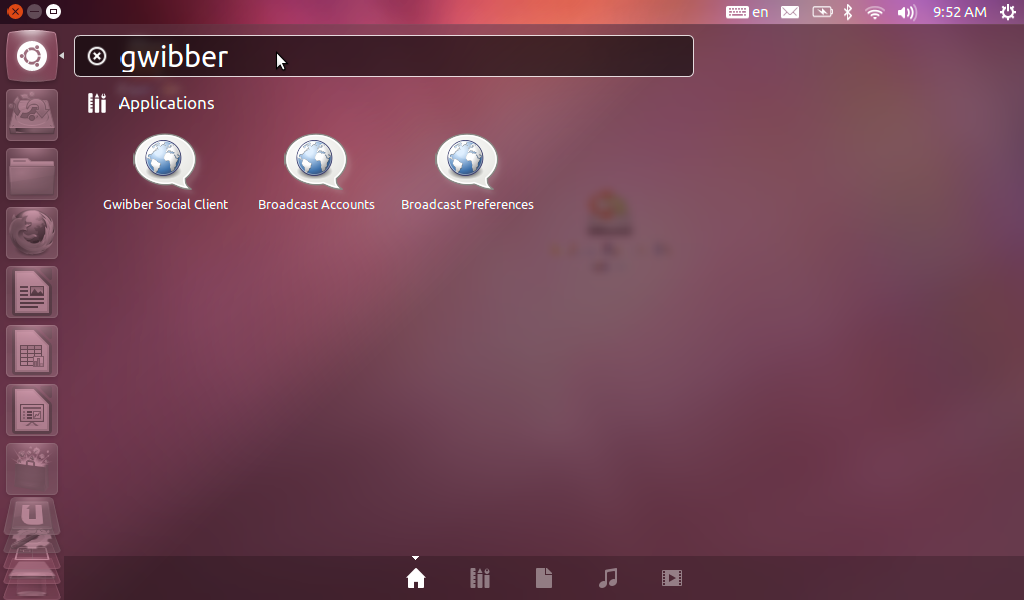
\includegraphics[width=300pt]{./images/basic-tasks/gwibber1.png}
	\caption{Launch Gwibber from the dash}	
	\label{fig:gwibber1}		
\end{figure}

\subsection*{Step 2.  Short tour through Gwibber's interface}

\par \noindent After you left click Gwibber's icon on a dash you are prompted with Gwibber's dialog boxes. See figure \ref{fig:gwibber2}. \\

\begin{figure}[h!]	
	\centering
	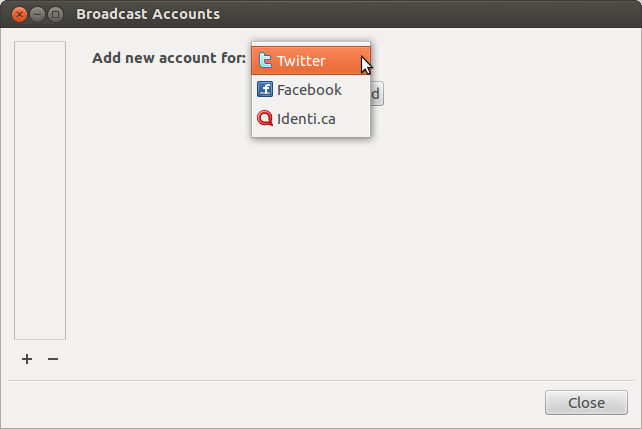
\includegraphics[width=200pt]{./images/basic-tasks/gwibber2.png}
	\caption{Gwibber web services}	
	\label{fig:gwibber2}		
\end{figure}

\par \noindent As you can see in figure \ref{fig:gwibber2},  this dialog box serves you to set up microblogging for the already mentioned web services like Twitter, Facebook etc. You will see that later on more detailed. 

\subsection*{Step 3.  Setting up the Gwibber for Twitter}

In figure \ref{fig:gwibber2} choose Twitter.  After you have chosen Twitter just left click the Add button. Next step is to start the authorization process with Twitter. Gwibber and Twitter have to be synchronized. Twitter has to authorize your access via Gwibber. To start the authorization you have to left click on the button Authorize. \\

\begin{figure}[h!]	
	\centering
	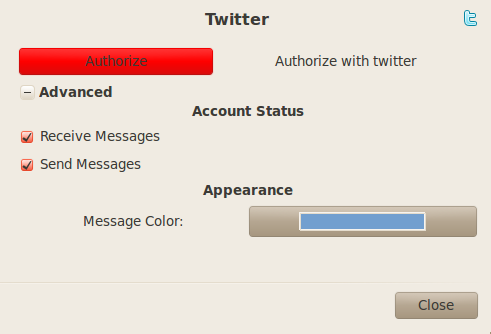
\includegraphics[width=200pt]{./images/basic-tasks/gwibber3.png}
	\caption{Configure account}	
	\label{fig:gwibber3}		
\end{figure}

\par \noindent As shown on in figure \ref{fig:gwibber3}, you can also set up others features like: receiving/sending messages, account color. After you have done that just click on the button Authorize. Further more you will be prompted with dialog box where you will have to enter your Twitter login credentials. See figure \ref{fig:gwibber4}. After you have entered your Twitter username and password you have to left click on the button Authorize app. \\

\begin{figure}[h!]	
	\centering
	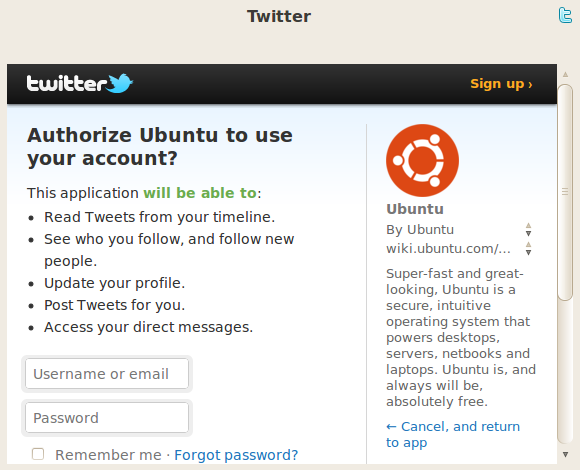
\includegraphics[width=200pt]{./images/basic-tasks/gwibber4.png}
	\caption{Twitter user credentials}	
	\label{fig:gwibber4}		
\end{figure}

\par \noindent You will have to wait until Twitter and Gwibber are synchronized. After synchronization is done you will be prompted that your account via Gwibber has been authorized. You can now close Gwibber's account setup dialog window.Now you can start messaging and looking at your tweet feed. (This will be shown on illustrations 8.1.10. to 8.1.12. \\

\par \noindent What you will see is:

\begin{itemize}
\item How does the interface looks like when you are reaching Twitter via Gwibber
\item How to send message via Gwibber
\item Tweet feed via Gwibber
\end{itemize}

\begin{figure}[ht!]	
		\centering		
		\subfloat[Gwibber Twitter interface]
		{ 	\label{fig:sound-menu} 	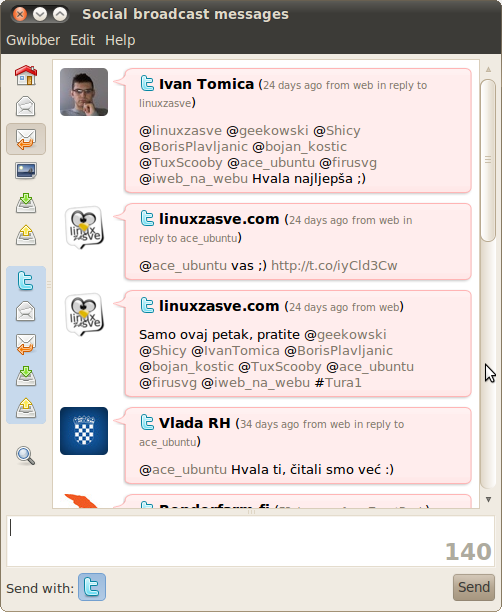
\includegraphics[width=200pt]{./images/basic-tasks/gwibber5.png} } 
		~ \hspace{0.5in}
		\subfloat[Gwibber Twitter tweet feed]
		{ 	\label{fig:messaging-menu} 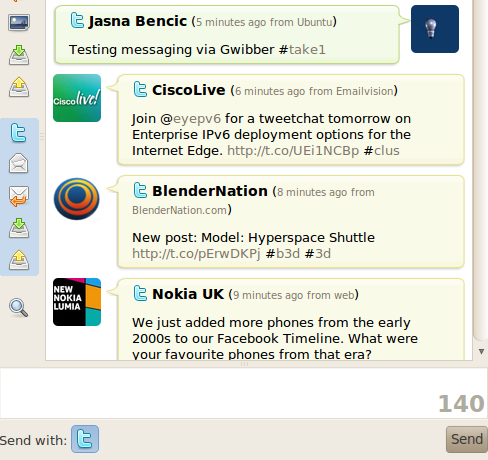
\includegraphics[width=200pt]{./images/basic-tasks/gwibber6.png}	}		
		\caption{Gwibber interface}
		\label{fig:gwibber}
\end{figure}


\section{Listening to music} \index{Music}
In Ubuntu, Rhythmbox is the default music player. You can launch the music player through the dash by searching for Rhythmbox. You also launch the music player using the sound menu. This is much quicker and easier to access at any time. This is illustrated in figure \ref{fig:play-music1}. The sound menu houses media applications and sound control settings. If you install other media applications such as Spotify, they will be automatically added to the sound menu. \\

\begin{figure}[h!]	
	\centering
	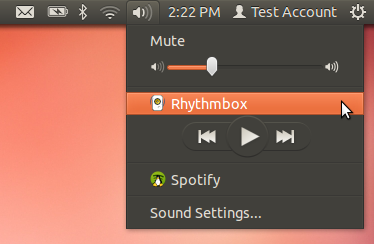
\includegraphics[width=150pt]{./images/basic-tasks/play-music1.png}
	\caption{Launch Rhythmbox from the sound menu}	
	\label{fig:play-music1}		
\end{figure}

\par \noindent The Rhythmbox music player can be seen in figure \ref{fig:play-music2}. It behaves like any standard media player. You can create playlists with your favourite music and save it for future playback. On first launch, Rhythmbox automatically starts importing all your music present in your music folder. You can also configure it to watch a specific folder for new music. Rhythmbox also includes the Ubuntu One music store where you can purchase music using your Ubuntu One account. If you do not have an account, you can create it easily. \\

\begin{figure}[h!]	
	\centering
	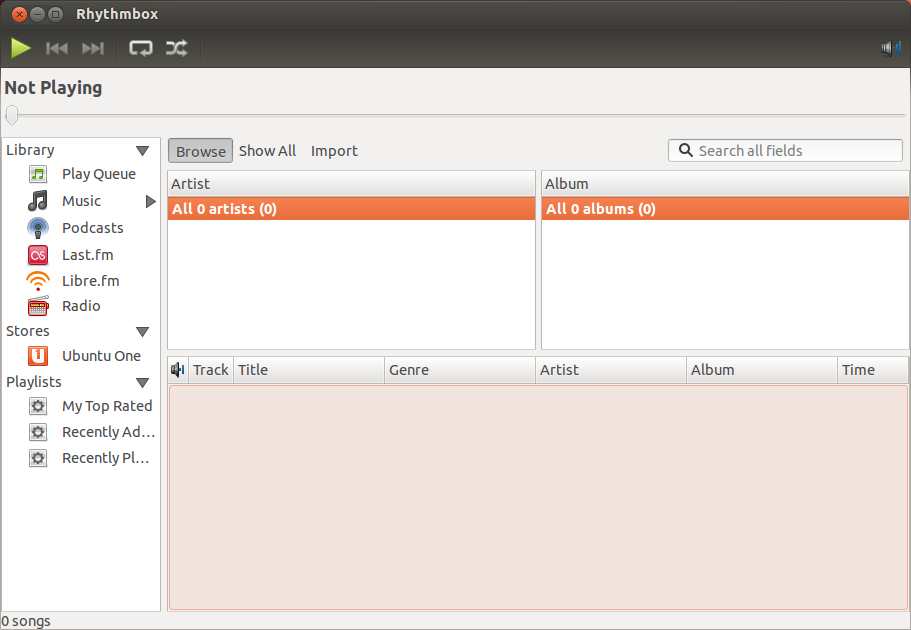
\includegraphics[width=250pt]{./images/basic-tasks/play-music2.png}
	\caption{Rhythmbox}	
	\label{fig:play-music2}		
\end{figure}

\par \noindent Since Rhythmbox can be easily accessed from the sound menu, you can also perform other operations from the sound menu directly. You can control all media operations such as Play, Pause, Forward, Reverse, choose playlist all within the sound menu without having to show the Rhythmbox interface. This allows for quick control of media playback. Imagine a scenario where you have several applications open. Instead of opening Rhythmbox and then controlling the music, you can just do this using the sound menu while Rhythmbox runs in the background. \\

\begin{figure}[h!]	
	\centering
	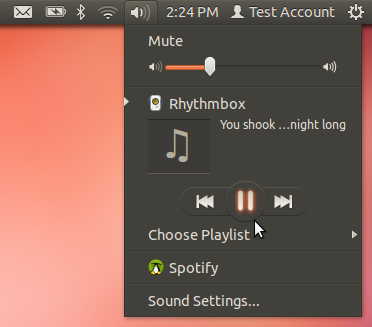
\includegraphics[width=150pt]{./images/basic-tasks/play-music3.png}
	\caption{Rhythmbox - Play/Pause}	
	\label{fig:play-music3}		
\end{figure}

\par \noindent \framebox[6.7in][l]{\parbox[l]{6.5in}{\textbf{Note}: When you click the close button, Rhythmbox does not quit but rather is still running in the background. This is intentional and intended to allow the user to continue with his work while the music player runs in the background. If you want to quit it, you have to choose quit from the Music menu.}} \\

\section{Editing Documents, Presentations, Spreadsheets} \label{sect:office}
Ubuntu by default comes with an office suite to help you get started straight away. You no longer need to worry about installing it after a fresh install of Ubuntu. LibreOffice is the office suite which is provided by default by Ubuntu. It is similar to Microsoft Office (Windows) or Office for Mac (Mac OS). Launching the office suite can be done by launching it from the dash or also from the launcher. LibreOffice Writer is similar to Microsoft Word, LibreOffice Calc is similar to Microsoft Excel and finally LibreOffice Impress is the counterpart of Microsoft Powerpoint. These programs are already present in your launcher and look like figure \ref{fig:office-icons}. \\

\begin{figure}[ht!]	
		\centering		
		\subfloat[]
		{ 	\label{fig:sound-menu} 	
\includegraphics[width=40pt]{./images/basic-tasks/document-icon.png} } 
		~ \hspace{0.5in}
		\subfloat[]
		{ 	\label{fig:messaging-menu} 
\includegraphics[width=40pt]{./images/basic-tasks/spreadsheet-icon.png}	}
		~ \hspace{0.5in}
		\subfloat[]
		{ 	\label{fig:messaging-menu} 
\includegraphics[width=40pt]{./images/basic-tasks/presentation-icon.png}	}
		\caption{Libreoffice icons}
		\label{fig:office-icons}
\end{figure}

\par \noindent LibreOffice is backed up by many companies, to name some of the prominent ones are Google, Red Hat, Novell etc. LibreOffice can handle all the documents created by Microsoft Office, so rest assured you will not run into collaboration problems (However LibreOffice doesn't have 100\% accuracy at importing or exporting Microsoft Office formats.). Writer, Calc and Impress can be seen in figure \ref{fig:edit-office}.

\begin{figure}[h!]	
	\centering
	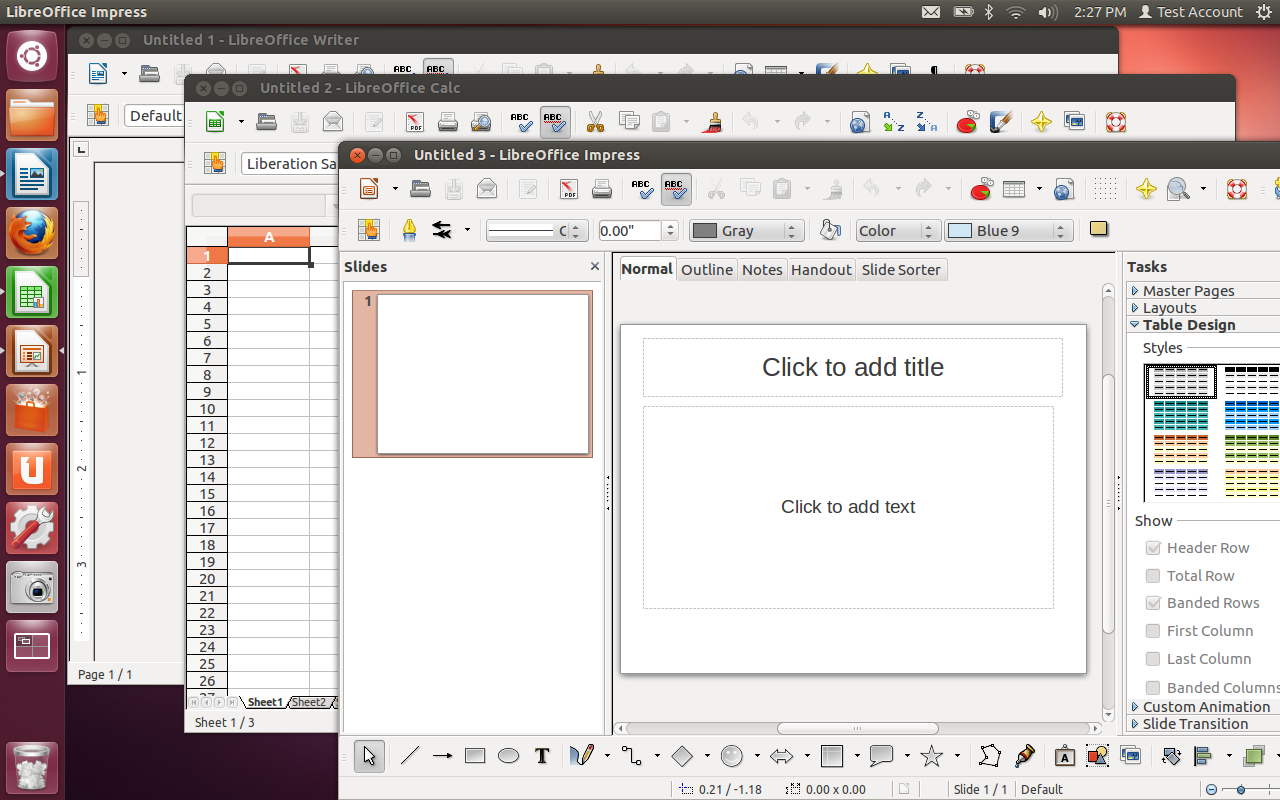
\includegraphics[width=300pt]{./images/basic-tasks/edit-office.png}
	\caption{Libreoffice}	
	\label{fig:edit-office}		
\end{figure}

\section{Setting up the internet} \index{Network}
Setting up the Internet under Ubuntu is pretty easy because everything works pretty much out of the box. You do not need to configure anything. The wireless networks detected are automatically shown in the networks menu in the top panel. The only think you are required to input are the password of the password protected networks. \\

\begin{figure}[h!]	
	\centering
	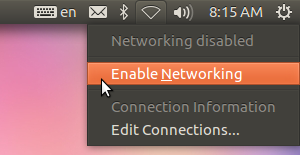
\includegraphics[width=150pt]{./images/basic-tasks/internet1.png}
	\caption{Network menu}	
	\label{fig:internet1}		
\end{figure}

\par \noindent However, sometimes you might want to edit your connections to change the settings. This can be done by clicking the Edit Connection menu items as seen in figure \ref{fig:internet2}.You will then be prompted with the Edit connection dialog window. See figure \ref{fig:internet3}. In the edit connections dialog window, you can configure the settings of any network profile that you wish to change. This includes all wired, wireless networks, mobile broadband, VPN and DSL. \\

\begin{figure}[ht!]	
		\centering		
		\subfloat[Edit Connections menu item]
		{ 	\label{fig:internet2} 	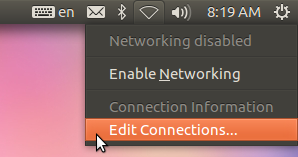
\includegraphics[width=150pt]{./images/basic-tasks/internet2.png} } 
		~ \hspace{0.5in}
		\subfloat[Edit Connections dialog window]
		{ 	\label{fig:internet3} 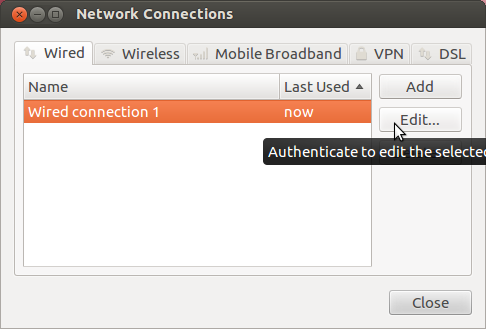
\includegraphics[width=200pt]{./images/basic-tasks/internet3.png}	}		
		\caption{Edit Connections}
		\label{fig:internet23}
\end{figure}

\par \noindent To edit/configure wired connection you have to left click on Edit button as shown in figure \ref{fig:internet3} so you could proceed to the wired connection set up. See figure \ref{fig:internet4}. As you can see in figure \ref{fig:internet4}, you can, 

\begin{itemize}
	\item Give the network connection a name.
	\item Decide if you want to connect to this particular network automatically when available.
	\item Edit the device MAC address  - this is already done by the system automatically. Note: wired connection is always named eth0 and wireless wlan0 by the system. If you will ever configure connection via Terminal you will need these labels. 
	\item Edit cloned MAC address
	\item Edit MTU (Maximum transmission unit)
\end{itemize}

\par \noindent Note: Network icon on the bar will change into two arrows pointing in two different directions when connection to the Internet is established. See figure \ref{fig:internet6}. \\

\begin{figure}[ht!]	
		\centering		
		\subfloat[Edit Connections menu item]
		{ 	\label{fig:internet4} 	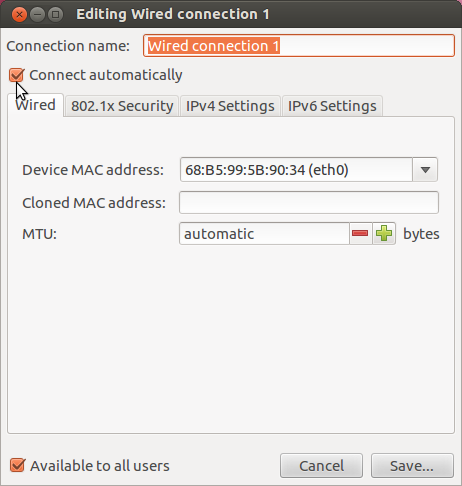
\includegraphics[width=200pt]{./images/basic-tasks/internet4.png} } 
		~ \hspace{0.5in}
		\subfloat[Wired connection complete]
		{ 	\label{fig:internet6} 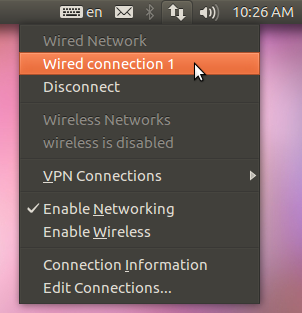
\includegraphics[width=150pt]{./images/basic-tasks/internet6.png}	}		
		\caption{Wired connection setup}
		\label{fig:internet46}
\end{figure}

\par \noindent Configuring wireless networks can be done in a similar fashion. You need to bring up the Edit connections dialog from the networks menu and then choose the wireless tab. Here you are shown the wireless networks you have previously connected to. The method is exactly similar to the wired approach described above and hence will not be repeated again. \\

\section{Printing documents, pictures} \index{Print}
You have read about the LibreOffice suit in section \ref{sect:office}. Printing documents in Ubuntu is very easy. Let's try printing a document using LibreOffice Writer. Open LibreOffice Writer and create a document. After that left click on the File menu and then click the Print submenu item. See figure \ref{fig:print1}. \\

\begin{figure}[h!]	
	\centering
	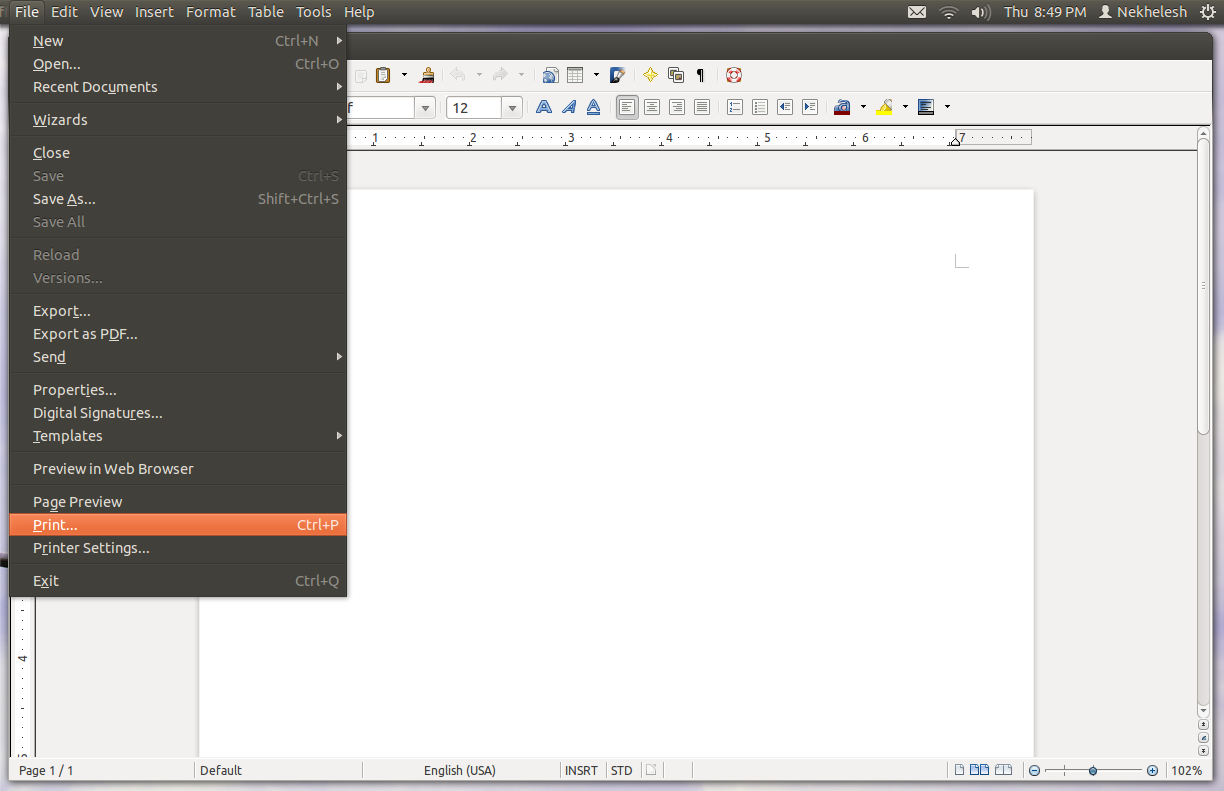
\includegraphics[width=300pt]{./images/basic-tasks/print1.png}
	\caption{Libreoffice Writer Print Menu}	
	\label{fig:print1}		
\end{figure}

\par \noindent Shortly you will be prompted with Print dialog window as seen in figure \ref{fig:print2}. \\

\begin{figure}[h!]	
	\centering
	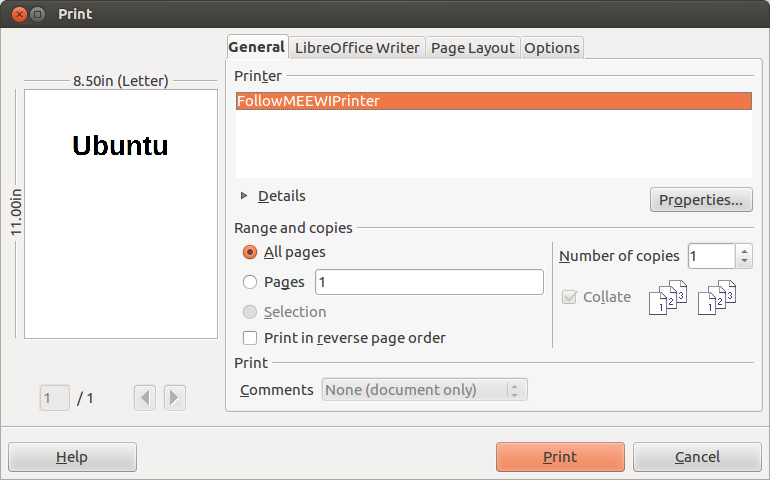
\includegraphics[width=200pt]{./images/basic-tasks/print2.png}
	\caption{Print Dialog}	
	\label{fig:print2}		
\end{figure}

\par \noindent Note: Most of the printers today work by the principle ``plug and play"  (hint USB).  Well, on some operating systems like Windows you may have to install a driver for a printer that you buy. You do not need to do that for Ubuntu, at least not for EPSON printers. Ubuntu recognizes them automatically at once just like the wireless networks in previous sections. All you have to do is wait a bit when you plug your printer into the computer until they synchronize. After that you can print as shown in figure \ref{fig:print2}. Procedure for printing pictures is the same as for printing documents.

\section{Composing Emails} \index{Email}
Mozilla Thunderbird is the default email client of Ubuntu. It boasts features such as Migration assistant to help you migrate from other desktop email clients, mail account setup wizard, tabbed interface and many other features. You can find more information about thunderbird \href{http://www.mozilla.org/en-US/thunderbird/features/}{here}. This section will show how to set up your e-mail and send a message. You can start Thunderbird by clicking on the e-mail icon on the top panel (shape of an envelope).  After that you have to left click on the sub menu item called Set up mail. See figure \ref{fig:thunderbird1}. \\

\begin{figure}[h!]	
	\centering
	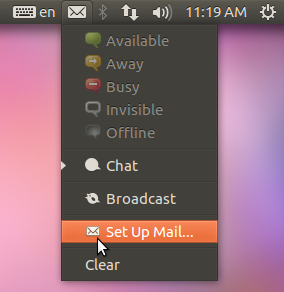
\includegraphics[width=150pt]{./images/basic-tasks/thunderbird1.png}
	\caption{Mozilla Thunderbird email client}	
	\label{fig:thunderbird1}		
\end{figure}

\par \noindent After that you will be prompted with Thunderbird's wizard for setting up an e-mail account. First step is to write your name,  e-mail address that you use and its password. (What ever you use: gmail, yahoo, hotmail etc.). See figure \ref{fig:thunderbird2}. Press Continue to proceed to the next step of the wizard.\\

\begin{figure}[h!]	
	\centering
	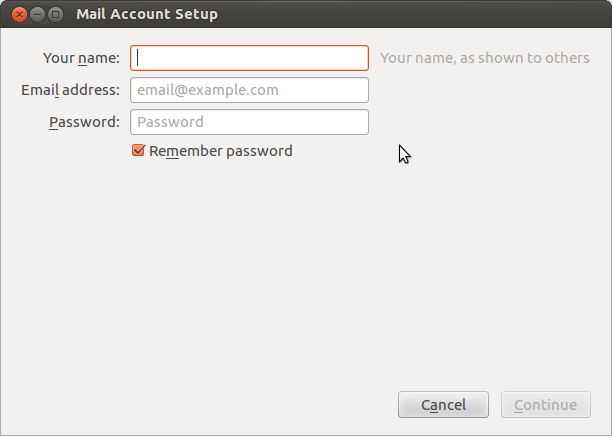
\includegraphics[width=200pt]{./images/basic-tasks/thunderbird2.png}
	\caption{Mail Account setup wizard}	
	\label{fig:thunderbird2}		
\end{figure}

\par \noindent Thunderbird will automatically set up the email account for you. Press the Create Account button on the wizard to complete the setup as seen in figure \ref{fig:thunderbird3}. After that you will have to wait for Thunderbird to synchronize all the emails and sets up you account. You no longer need to access your email from a web interface such as gmail.com or hotmail.com. You can access all your email right from your desktop. \\

\begin{figure}[h!]	
	\centering
	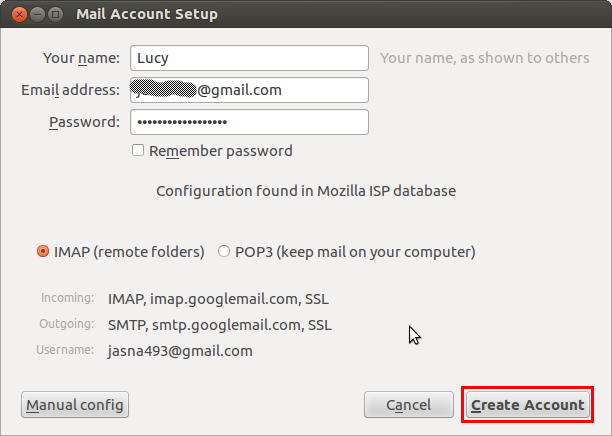
\includegraphics[width=200pt]{./images/basic-tasks/thunderbird3.png}
	\caption{Mail Account setup wizard}	
	\label{fig:thunderbird3}		
\end{figure}

\par \noindent You will then be prompted with Thunderbird's System Integration dialog box, where you will be asked for what you want to use Thunderbird by default. In this case it is just E-mail). See figure \ref{fig:thunderbird4}. Now you are ready to compose a new message. \\

\begin{figure}[h!]	
	\centering
	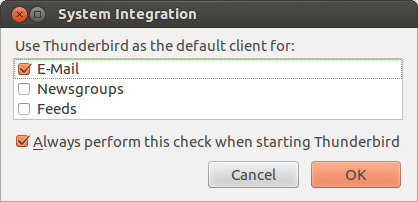
\includegraphics[width=200pt]{./images/basic-tasks/thunderbird4.png}
	\caption{System Integration dialog}	
	\label{fig:thunderbird4}		
\end{figure}

\par \noindent To compose a new message you have to click on a Write new message command as shown in figure \ref{fig:thunderbird5}. After that you will be prompted with a familiar interface for composing an email as seen in figure \ref{fig:thunderbird6}.

\begin{figure}[h!]	
	\centering
	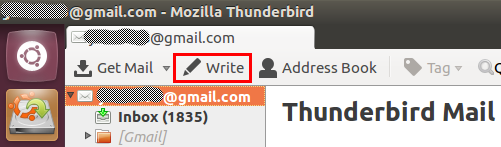
\includegraphics[width=150pt]{./images/basic-tasks/thunderbird5.png}
	\caption{Create new message}	
	\label{fig:thunderbird5}		
\end{figure}

\begin{figure}[h!]	
	\centering
	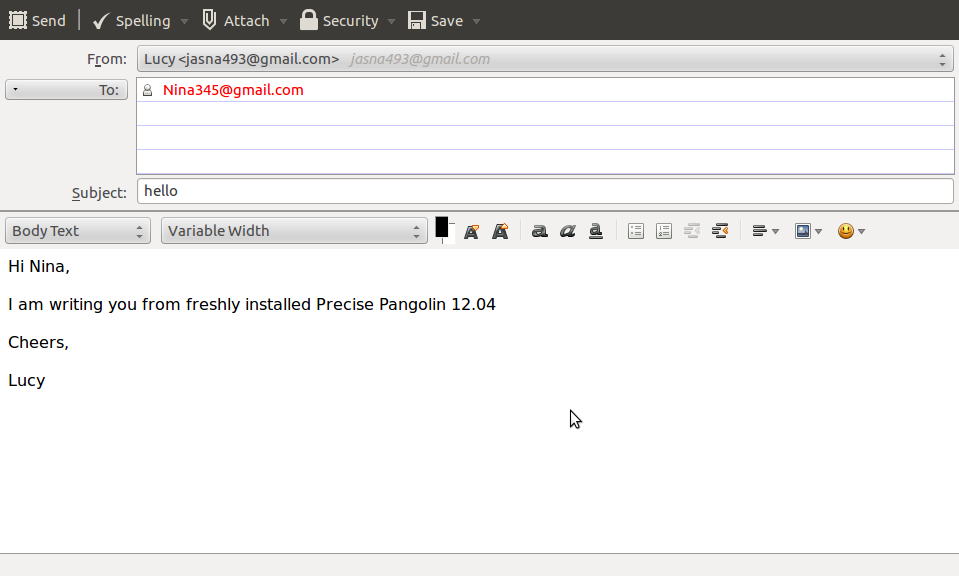
\includegraphics[width=300pt]{./images/basic-tasks/thunderbird6.png}
	\caption{Compose new message}	
	\label{fig:thunderbird6}		
\end{figure}

\section{Browsing the web} \index{Browse}
Mozilla Firefox is the default web browser of Ubuntu. Firefox is an open source application which is cross-platform, meaning you can use it other operating systems such as Windows and Mac OS. It is the second most popular web browser in the world. You can launch Firefox either from the launcher or the dash. You can see the Firefox interface in figure \ref{fig:firefox2}. \\

\begin{figure}[h!]	
	\centering
	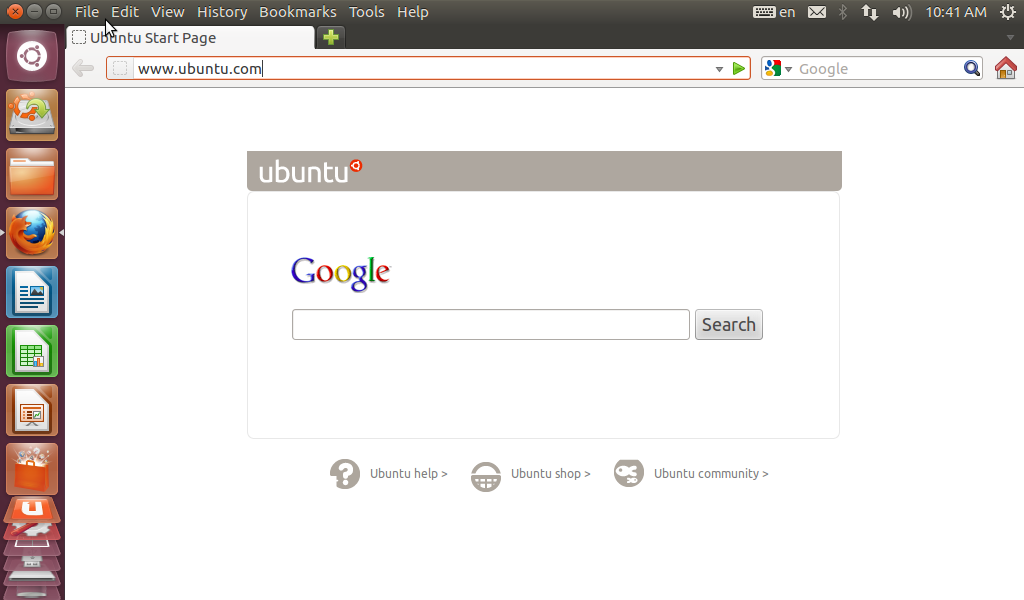
\includegraphics[width=300pt]{./images/basic-tasks/firefox2.png}
	\caption{Mozilla Firefox web browser}	
	\label{fig:firefox2}		
\end{figure}

\par \noindent Firefox supports tabbed browsing, synchronization with other devices and provides support to customize your browser using add-ons which can be downloaded from their website at \href{www.firefox.com}{firefox.com}. Updates to Firefox are automatically done by Ubuntu to ensure that you have the latest modern web browser on your system.

\newpage
\section{Sharing files with other users} \index{Ubuntu One} \index{Personal Cloud} \index{Web Storage}
Ubuntu 12.04 by default comes with the popular file sharing program called Ubuntu One. It is a personal storage space (cloud) on the web to store files, music and videos. Every Ubuntu user is entitled to an Ubuntu One account which by default offers 5 GB storage space. You are required to create a Ubuntu account which can also be used for other purposes like Launchpad, Ubuntu Software Center, Ubuntu Shop and other Ubuntu services. Ubuntu One offers the following features,

\begin{itemize}
	\item 5 GB free storage space on the web (cloud storage)
	\item Share and access your files from multiple devices like your computer, phones etc.
	\item Stream your music across all your portable devices.
	\item Available for many platforms
\end{itemize}

\par \noindent Ubuntu One is available on many platforms like Windows, Android, iPhone, iPad and also expected to arrive for the Mac OS at the time of writing this manual. This way you can share files without any hassle among these devices through Ubuntu One. Ubuntu One can be compared to other online file storage applications like iCloud, Dropbox etc. Ubuntu One also also provides music streaming feature. You can wirelessly sync your music to your portable devices to have music on the go. And since Ubuntu One is available for Android and iPhone, you have access to the entire music collection present on your computer at home.\\

\par \noindent Let's consider a scenario where you have multiple laptop running Windows operating system, Ubuntu and also other portable devices such as you Android phone. Ubuntu One allows you to share your files to all these devices. So instead of having to copy/paste files on to each of these devices individually, you can instead just save the file in your Ubuntu One web storage and these will automatically be available on all your devices. In this section, instructions to create an Ubuntu One account and share files with other users will be shown. 

\subsection*{Setting up Ubuntu One}

\par \noindent Click on the Ubuntu One application icon on the launcher. It looks like figure \ref{fig:share1}. This icon also displays the sync status once the configuration process is complete.

\begin{figure}[h!]	
	\centering
	
\includegraphics[width=40pt]{./images/basic-tasks/share1.png}
	\caption{Ubuntu One application icon}	
	\label{fig:share1}		
\end{figure}

\par \noindent On clicking the icon for the very first time on a new Ubuntu install, you are presented with the Ubuntu One install wizard as shown in figure \ref{fig:share2}. Click the install button to start the installation. 

\begin{figure}[h!]	
	\centering
	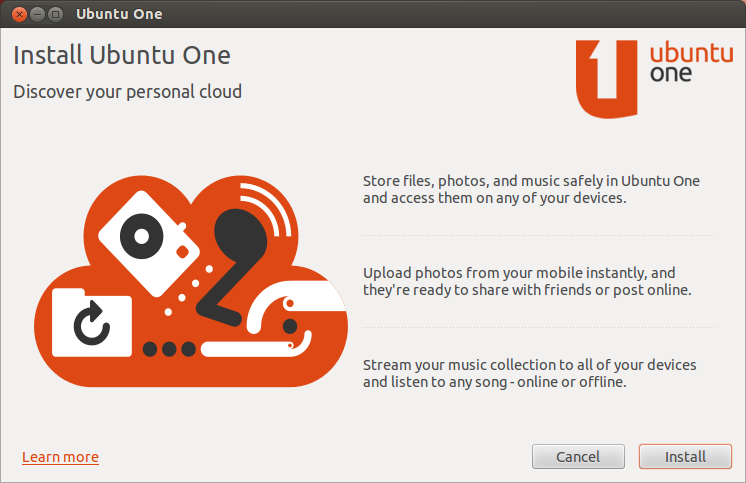
\includegraphics[width=300pt]{./images/basic-tasks/share2.png}
	\caption{Ubuntu One install wizard}	
	\label{fig:share2}		
\end{figure}

\par \noindent Once the installation is complete, you are shown the setup wizard where the steps required to complete the initial Ubuntu One configuration is shown. Since the installation is complete, the remaining steps include signing in to your Ubuntu One account, choosing the folders to sync and then finally synchronisation itself. First, you can either choose to login into an existing account or create a new account. Both choices will be explained below. \\

\begin{figure}[h!]	
	\centering
	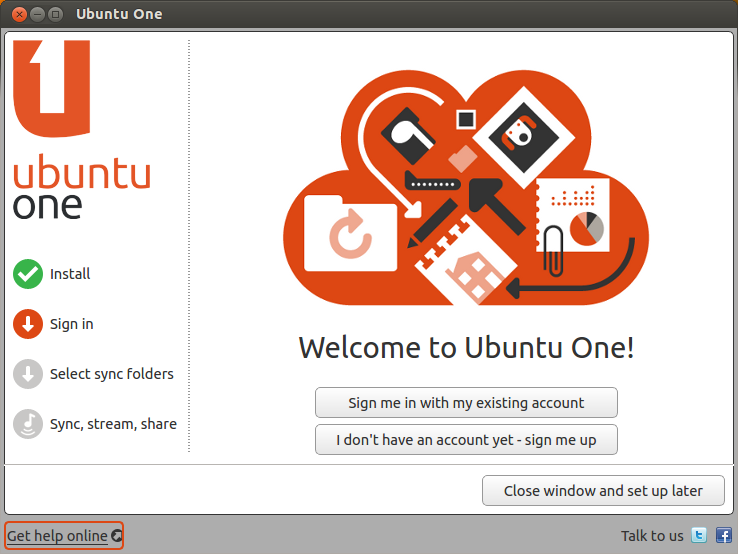
\includegraphics[width=300pt]{./images/basic-tasks/share3.png}
	\caption{Ubuntu One account setup}	
	\label{fig:share3}		
\end{figure}

\par \noindent Let's first start with signing in to an existing account. When you click on \textit{Sign me in with my existing account}, you are presented with a dialog window where you enter your Ubuntu One user credentials as shown in figure \ref{fig:share4}. Once you are done, click Sign In. \\

\begin{figure}[h!]	
	\centering
	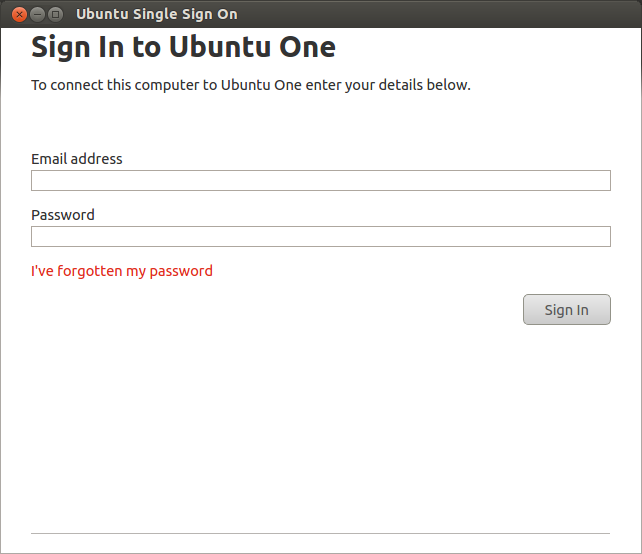
\includegraphics[width=300pt]{./images/basic-tasks/share4.png}
	\caption{Ubuntu One user credentials}	
	\label{fig:share4}		
\end{figure}

\newpage
\par \noindent In this step, you can choose which folders you want to sync from the cloud (web storage) to your computer. This is useful to only sync the required files. For instance, on your mobile phone you might not want to sync all the files but rather just selected music files perhaps. Once done, click the Next button.\\

\begin{figure}[h!]	
	\centering
	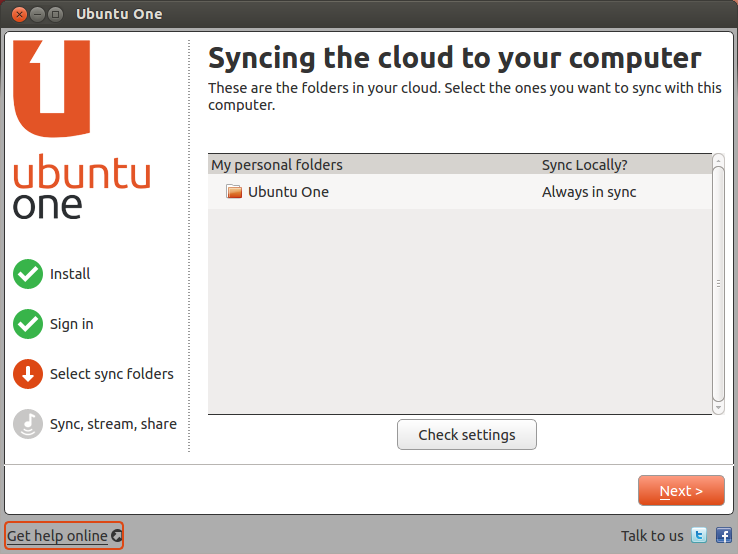
\includegraphics[width=300pt]{./images/basic-tasks/share8.png}
	\caption{Syncing cloud to computer}	
	\label{fig:share8}		
\end{figure}

\par \noindent In the final step, you can choose which folders you want to sync from your device to the cloud storage. You might be interested to only sync important files to the cloud to save space. You can choose any folder that you want from your computer. Any changes that you make in that folder will be automatically synchronised to the cloud. Hence all your devices which are connected to Ubuntu One will always be up to date. \\

\begin{figure}[h!]	
	\centering
	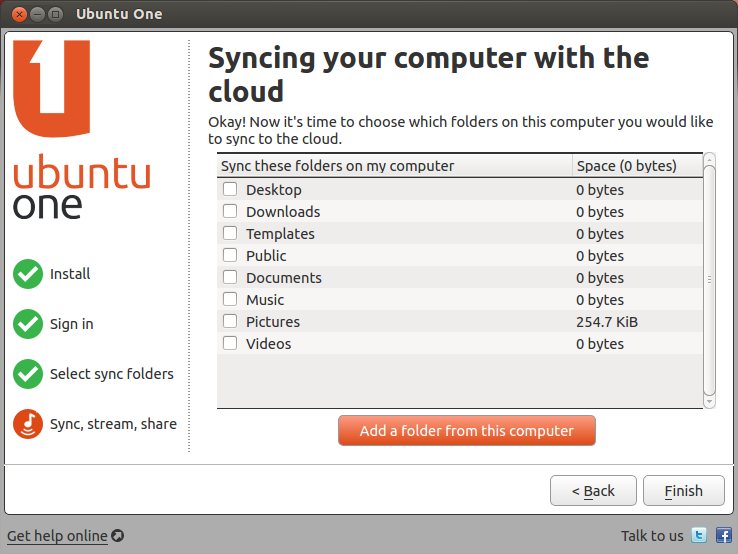
\includegraphics[width=300pt]{./images/basic-tasks/share9.png}
	\caption{Syncing computer to cloud}	
	\label{fig:share9}		
\end{figure}

\newpage
\par \noindent Let's now return to the step where you have to create a new Ubuntu One account. If you clicked \textit{I don't have an account yet- sign me up} in figure \ref{fig:share3}, you are then presented with a form, where you can fill in all the required information to create a Ubuntu One account. This is easy to follow and the steps are pictorially represented below in figures \ref{fig:share5} and \ref{fig:share7}. \\

\begin{figure}[h!]	
	\centering
	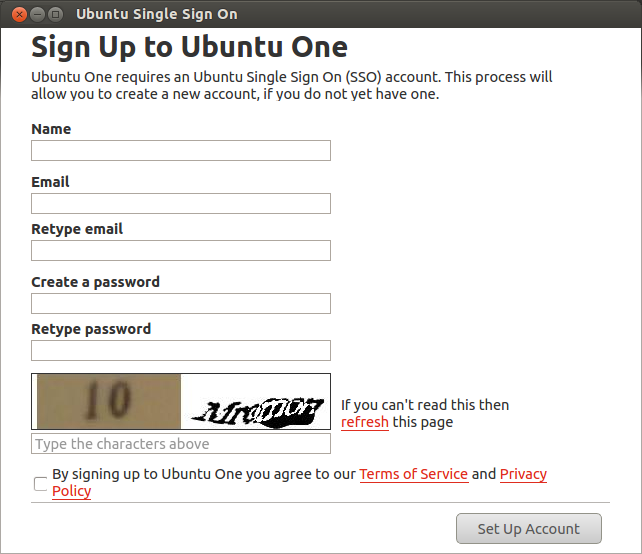
\includegraphics[width=300pt]{./images/basic-tasks/share5.png}
	\caption{Enter user credentials}	
	\label{fig:share5}		
\end{figure}

\begin{figure}[h!]	
	\centering
	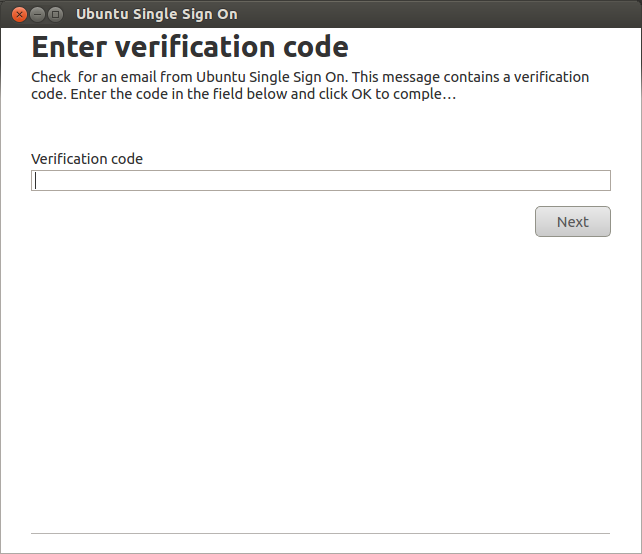
\includegraphics[width=300pt]{./images/basic-tasks/share7.png}
	\caption{Enter verification code}	
	\label{fig:share7}		
\end{figure}

\newpage
\par \noindent When all the steps are complete, you are finally shown the Ubuntu One control panel. This is the central place from where you can manage all your Ubuntu One settings. You can choose the download/upload speeds, personal details, choose which folders to sync etc. Try to spend some time getting acquainted with the Ubuntu One control panel. It will come handy in the future when you want to change some settings. You can see the Ubuntu One control panel in figure \ref{fig:share10}. \\

\begin{figure}[h!]	
	\centering
	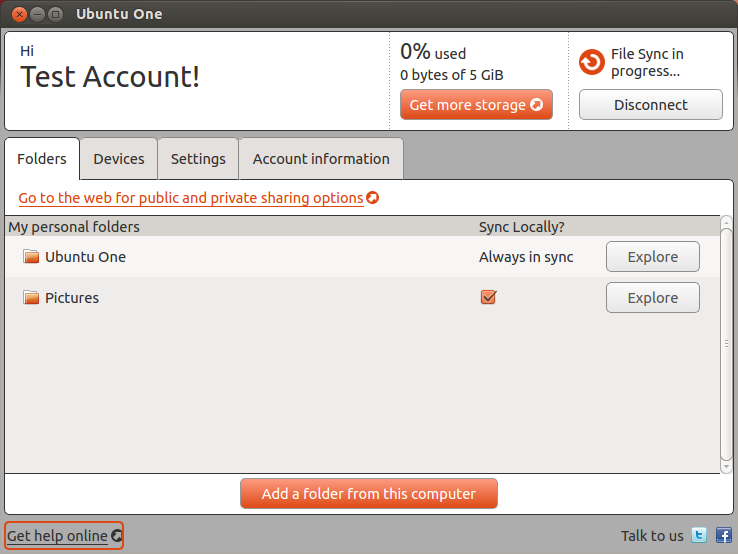
\includegraphics[width=300pt]{./images/basic-tasks/share10.png}
	\caption{Ubuntu One control panel}	
	\label{fig:share10}		
\end{figure}

\par \noindent Now that Ubuntu One has been configured, let's see how to share files, understand file sync status and also publish files. The methods below can also be done using the web interface which can be accessed at \href{https://one.ubuntu.com/}{one.ubuntu.com}.

\subsection*{Sync Status and Publishing Files} \index{Ubuntu One!Publish Files}
Open the file manager and click on the Ubuntu One bookmark shown on the left column. In the Ubuntu One folder, you will find all the files which are synced to this device (computer, phone etc).  It important to see what icons are used to represent the sync status first. The files in the Ubuntu One will have these emblems on each file and folder icon to indicate their syncing status. 

\begin{figure}[ht!]	
		\centering		
		\subfloat[Updating]
		{ 	\label{fig:updating_emblem} 	
\includegraphics[width=40pt]{./images/basic-tasks/updating_emblem.png} } 
		~ \hspace{0.5in}
		\subfloat[Synced]
		{ 	\label{fig:synced_emblem} 
\includegraphics[width=40pt]{./images/basic-tasks/synced_emblem.png}	}
		~ \hspace{0.5in}
		\subfloat[Unsynced]
		{ 	\label{fig:unsynced_emblem} 
\includegraphics[width=40pt]{./images/basic-tasks/unsynced_emblem.png}	}		
		\caption{Syncing Status}
		\label{fig:syncing_status}
\end{figure}

\par \noindent If you wanted to share a file to anyone on the internet, you can do so by using the publishing feature of Ubuntu One. When you publish a file, you are given a web link to the file. You can share this web link anywhere to anyone to access your file. To publish a file, right-click the file that you want to publish, under Ubuntu One, click publish as shown in figure \ref{fig:publish}. You are then provided with a web link which you can then use to let others see the file.  \\

\begin{figure}[h!]	
	\centering
	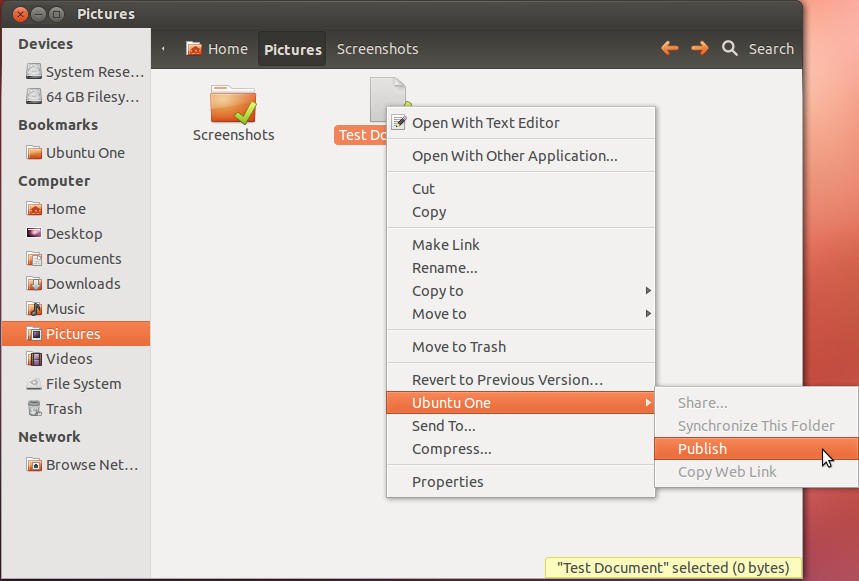
\includegraphics[width=300pt]{./images/basic-tasks/publish.png}
	\caption{Publish a file}	
	\label{fig:publish}		
\end{figure}

\par \noindent \framebox[6.7in][l]{\parbox[l]{6.5in}{\textbf{Note}: When you publish a file, other users can only view the file but not perform any changes to it, and hence no unauthorised changes are reflected on your cloud storage.}} \\

\subsection*{Sharing Folders with other users} \index{Ubuntu One!Share Folders}
To share files with other users, it is necessary to use the web interface since currently at the time of writing this manual, it is not possible to share a file or folder using the file manager. You can access the web interface at \href{https://one.ubuntu.com/}{one.ubuntu.com}. In the web interface, click on the file tab. Here you can see all the files stored in Ubuntu One across all your devices. Click on the more link at the right and choose share this folder. This is shown in figure \ref{fig:share-folder}. \\

\begin{figure}[h!]	
	\centering
	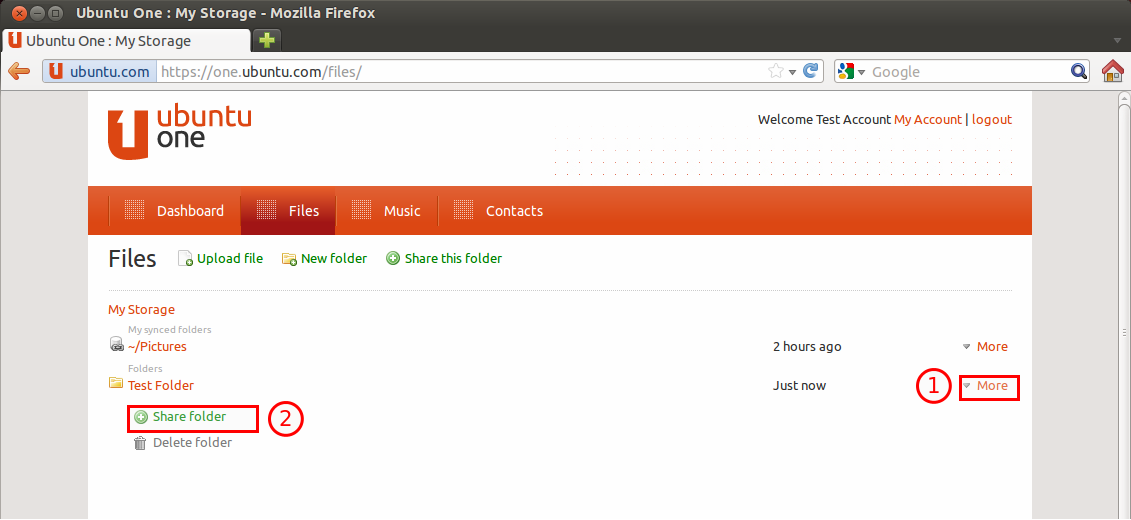
\includegraphics[width=400pt]{./images/basic-tasks/share-folder.png}
	\caption{Share a folder}	
	\label{fig:share-folder}		
\end{figure}

\par \noindent On clicking the share folder, you are presented with a dialog box where you need to enter the user's ubuntu one email address. You can also choose to give write permissions to the user. This is shown in figure \ref{fig:share-folder2}.

\begin{figure}[h!]	
	\centering
	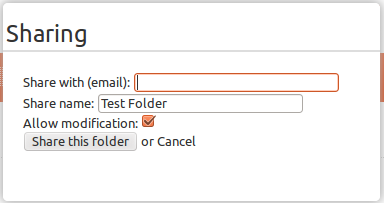
\includegraphics[width=200pt]{./images/basic-tasks/share-folder2.png}
	\caption{Share options}	
	\label{fig:share-folder2}		
\end{figure}

\par \noindent The other user will get an email notification asking to accept the invitation to the shared folder. This way you can collaborate with other users using Ubuntu One.

\section{Playing Games} \index{Games}
Ubuntu comes with some pre-installed games such as Mines, Mahjongg, Sudoku etc. providing ways to kill time. You can see all the games installed on your computer using the dash. Proceed to the application lens, click on the filter and choose games. The applications will now all the games installed on your system. This is illustrated in figure \ref{fig:play-games1}. \\

\begin{figure}[h!]	
	\centering
	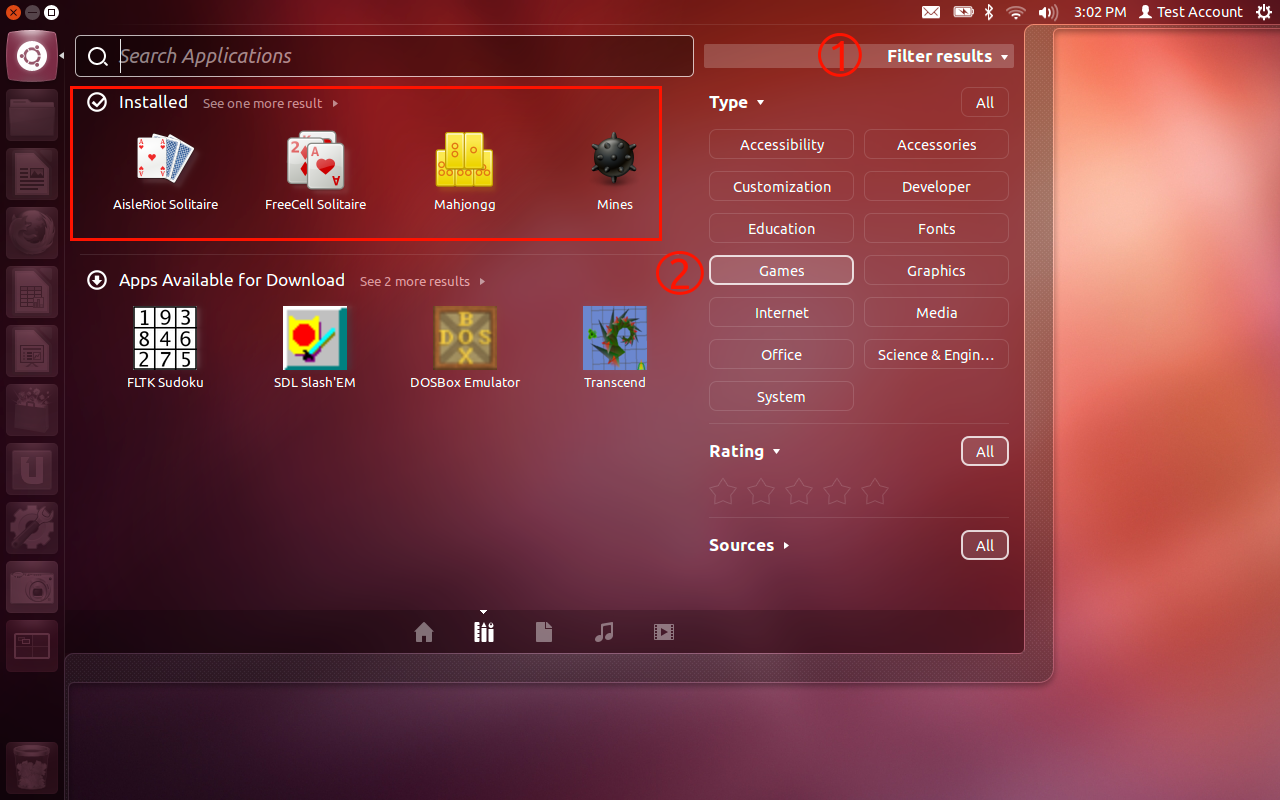
\includegraphics[width=300pt]{./images/basic-tasks/play-games1.png}
	\caption{Launch games from the dash}	
	\label{fig:play-games1}		
\end{figure}

\par \noindent You can install more games from the Ubuntu Software Center.